\section{Semaine 5 : 06/03/2023 - 10/03/2023}
\graphicspath{{semaines/semaine_5/images/}}

\begin{abstract}
	Pendant cette semaine, on a globalement cherché à comprendre les problèmes liés à l'interpolation de $\phi$. On s'est donc concentré sur la précision de la correction lorsque l'on prend la solution analytique en entrée. On a testé avec deux solutions analytiques : la solution trigonométrique considérées précédemment et une solution polynomiale. La partie où l'on va utilisé le FNO sera considéré dans un second temps.
\end{abstract}

Dans toute la suite, les erreurs calculées en norme L2 sont les erreurs relatives calculées de la manière suivante :

$$||y_{true}-y_{pred}||^2_{L^2(\Omega_h),rel}=\frac{\int_{\Omega_h}(y_{true}-y_{pred})^2}{\int_{\Omega_h}y_{true}^2}$$

\subsection{Solution analytique trigonométrique}

On considère la solution analytique (au problème de Poisson avec conditions de Dirichlet homogène) :
$$u_{ex}(x,y) = \frac{1}{\sin\left(k_1\frac{\pi}{2}\right)}\times\sin\left(k_1\frac{\pi}{2}\left(\frac{4}{\sqrt{2}}\right)^2\left((x-0.5)^2+(y-0.5)^2\right)\right)\times\cos\left(\frac{\pi}{2}\left(\frac{4}{\sqrt{2}}\right)^2\left((x-0.5)^2+(y-0.5)^2\right)\right)\,, $$ 

avec $k_1 \sim \mathcal{U}([0.1,1])$.

\subsubsection*{Extrapolate en faisant varier nb\_vert}

On va calculer l'erreur en norme L2 pour différents degré d'extrapolation (de 2 à 4) et pour différents nb\_vert. On calculera les facteurs multiplicatifs entre les résultats obtenus pour différentes valeurs  de nb\_vert.

Attention : Les résultats obtenus pour chaque valeur de nb\_vert n'ont pas été calculés pour les mêmes valeurs du paramètres $k_1$. 

\begin{minipage}{\linewidth}
	\centering
	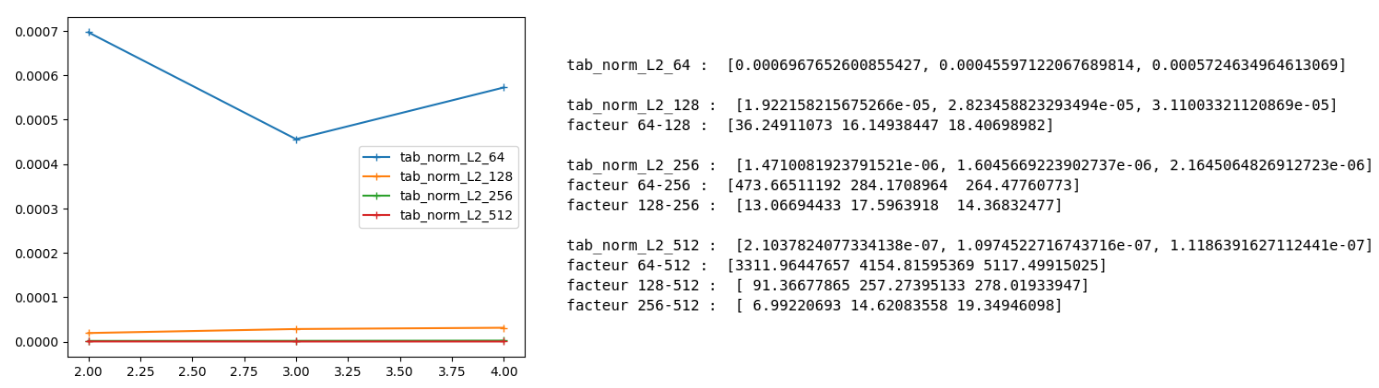
\includegraphics[width=0.9\linewidth]{test1_trigo.png}
\end{minipage}

\subsubsection*{Comparaison avec PhiFEM}

On veut comparer les erreurs en normes L2 pour différents degré d'interpolation. On fait une moyenne des résultats obtenus sur  10 valeurs de paramètres $k_1$ (nb\_data=10). Les comparaisons entre PhiFEM et la correction (pour différents degré d'interpolation) sont effectuées pour les mêmes valeurs de paramètres. On testera avec nb\_vert=64 (à gauche) et nb\_vert=128 (à droite). 

\begin{minipage}{\linewidth}
	\centering
	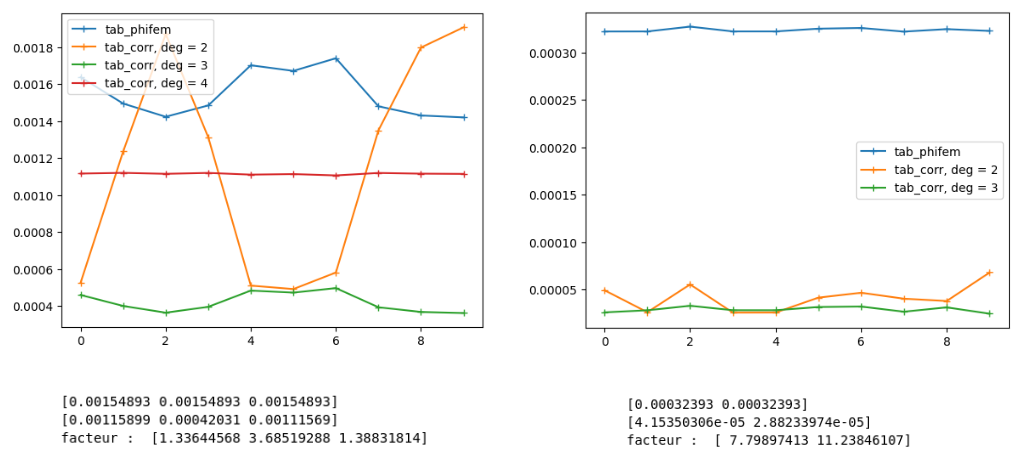
\includegraphics[width=0.7\linewidth]{test2_trigo.png}
\end{minipage}

\subsubsection*{Stratégie P1 fin -> Pk grossier}

Méthode précédente (avec le extrapolate) : On part d'une grille nb\_vert $\times$ nb\_vert. On associe alors les valeurs au noeuds aux valeurs des degré de liberté $\mathbb{P}^1$ puis on va extrapoler en $\mathbb{P}^k$ nb\_vert $\times$ nb\_vert. 

$$[\bar{\phi}=\phi w]_{ij \; grossier} \quad \longrightarrow \quad \mathbb{P}^1_{\; grossier} \quad \overset{extra}{\longrightarrow} \quad \mathbb{P}^k_{\; grossier}$$

On va considérer ici une nouvelle méthode : On part d'une grille fine nb\_vert\_fine $\times$ nb\_vert\_fine. On associe alors les valeurs aux noeuds aux valeurs des degrés de liberté $\mathbb{P}^1$ (nb\_vert\_fine $\times$ nb\_vert\_fine) puis on  interpole en $\mathbb{P}^k$ nb\_vert\_coarse $\times$ nb\_vert\_coarse. 

$$[\bar{\phi}=\phi w]_{ij \; fin} \quad \longrightarrow \quad \mathbb{P}^1_{\; fin} \quad \overset{inter}{\longrightarrow} \quad \mathbb{P}^k_{\; grossier}$$

On effectuera plusieurs comparaisons (avec nb\_data=10) :

\begin{enumerate}[label=\textbullet]
	\item \textbf{1er test : } 
	
	\begin{minipage}{0.48\linewidth}
		On va comparer les méthodes suivantes :
		$$[\bar{\phi}=\phi w]_{ij \; 64} \quad \longrightarrow \quad \mathbb{P}^1_{\; 64} \quad \overset{extra^3}{\longrightarrow} \quad \mathbb{P}^3_{\; 64}$$
		$$[\bar{\phi}=\phi w]_{ij \; 256} \quad \longrightarrow \quad \mathbb{P}^1_{\; 256} \quad \overset{inter}{\longrightarrow} \quad \mathbb{P}^2_{\; 64}$$
		$$[\bar{\phi}=\phi w]_{ij \; 256} \quad \longrightarrow \quad \mathbb{P}^1_{\; 256} \quad \overset{inter}{\longrightarrow} \quad \mathbb{P}^3_{\; 64}$$
	\end{minipage}
	\begin{minipage}{0.48\linewidth}
		\centering
		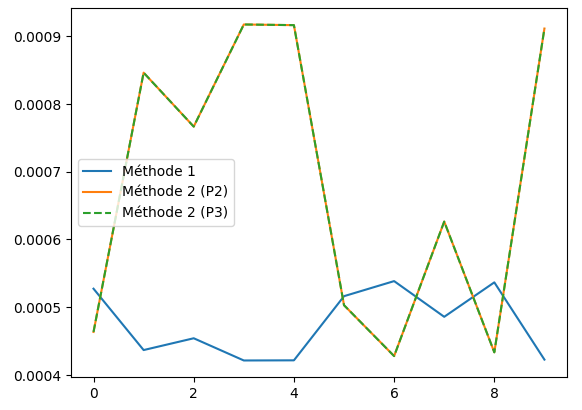
\includegraphics[width=\linewidth]{test3_trigo_1.png}
	\end{minipage}

	(Les courbes orange et verte sont très proches.)

	\item \textbf{2ème test : } 
	
	\begin{minipage}{0.48\linewidth}
		On va comparer les méthodes suivantes :
		$$[\bar{\phi}=\phi w]_{ij \; 256} \quad \longrightarrow \quad \mathbb{P}^1_{\; 256} \quad \overset{inter}{\longrightarrow} \quad \mathbb{P}^2_{\; 64}$$
		$$[\bar{\phi}=\phi w]_{ij \; 512} \quad \longrightarrow \quad \mathbb{P}^1_{\; 512} \quad \overset{inter}{\longrightarrow} \quad \mathbb{P}^3_{\; 64}$$
	\end{minipage}
	\begin{minipage}{0.48\linewidth}
		\centering
		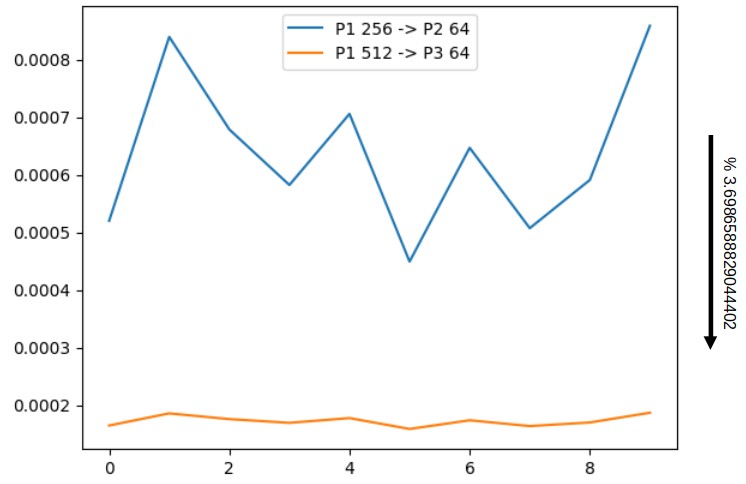
\includegraphics[width=\linewidth]{test3_trigo_2.png}
	\end{minipage}

	\item \textbf{3ème test : } 
	
	\begin{minipage}{0.48\linewidth}
		On va comparer les méthodes suivantes :
		$$[\bar{\phi}=\phi w]_{ij \; 256} \quad \longrightarrow \quad \mathbb{P}^1_{\; 256} \quad \overset{inter}{\longrightarrow} \quad \mathbb{P}^2_{\; 64}$$
		$$[\bar{\phi}=\phi w]_{ij \; 512} \quad \longrightarrow \quad \mathbb{P}^1_{\; 512} \quad \overset{inter}{\longrightarrow} \quad \mathbb{P}^3_{\; 64}$$
		$$[\bar{\phi}=\phi w]_{ij \; 512} \quad \longrightarrow \quad \mathbb{P}^1_{\; 512} \quad \overset{inter}{\longrightarrow} \quad \mathbb{P}^3_{\; 128}$$
		$$[\bar{\phi}=\phi w]_{ij \; 1024} \quad \longrightarrow \quad \mathbb{P}^1_{\; 1024} \quad \overset{inter}{\longrightarrow} \quad \mathbb{P}^3_{\; 256}$$
	\end{minipage}
	\begin{minipage}{0.48\linewidth}
		\centering
		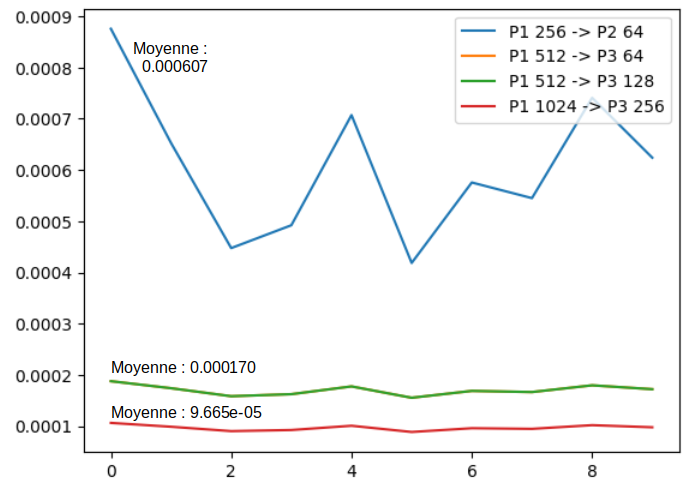
\includegraphics[width=\linewidth]{test3_trigo_3.png}
	\end{minipage}
	
	(Les courbes orange et verte sont très proches.)

\end{enumerate}

\subsection{Solution analytique polynomiale}

On considère la solution analytique (au problème de Poisson avec conditions de Dirichlet homogène) :

$$u_{ex}(x,y) = (1+k_1*x+k_2*y+x^2+y^2+x^3+y^3)\times\phi(x,y)$$

avec $k_1,k_2\sim\mathcal{U}(1,5)$

On va effectuer exactement les mêmes tests que dans le cas trigonométrique.

\subsubsection*{Extrapolate en faisant varier nb\_vert}

\begin{minipage}{\linewidth}
	\centering
	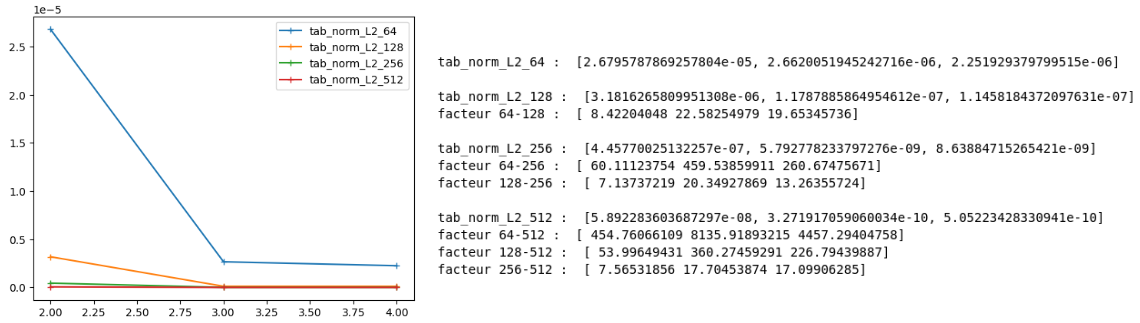
\includegraphics[width=\linewidth]{test1_poly.png}
\end{minipage}

\begin{minipage}{0.48\linewidth}
	\centering
	\subsubsection*{Comparaison avec PhiFEM}
	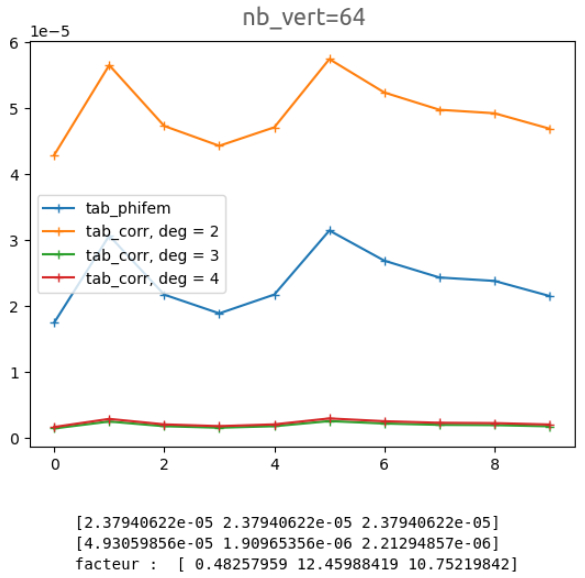
\includegraphics[width=0.85\linewidth]{test2_poly_1.png}
	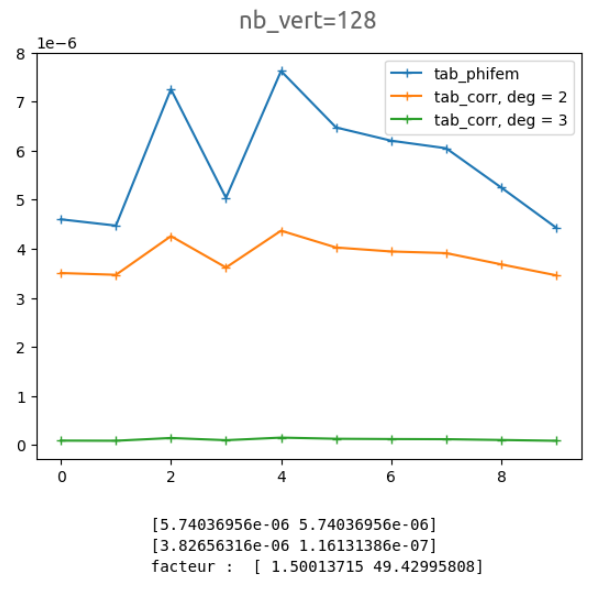
\includegraphics[width=0.85\linewidth]{test2_poly_2.png}
\end{minipage}
\begin{minipage}{0.48\linewidth}

	\centering
	\subsubsection*{Stratégie P1 fin -> Pk grossier}
	\textbf{1er test :} \\
	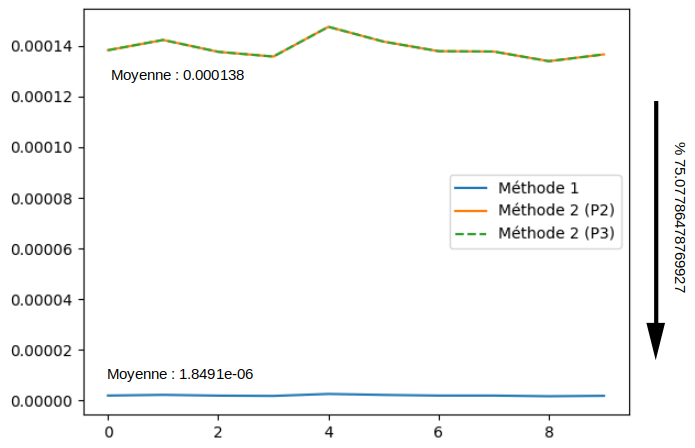
\includegraphics[width=0.8\linewidth]{test3_poly_1.png} \\
	\textbf{2ème test :} \\
	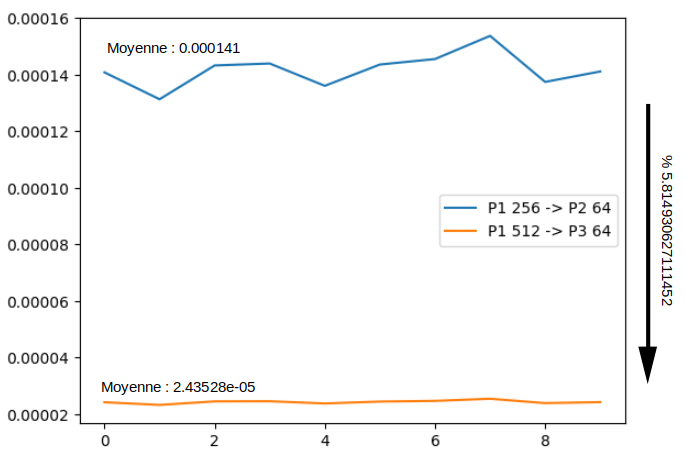
\includegraphics[width=0.8\linewidth]{test3_poly_2.png} \\
	\textbf{3ème test :} \\
	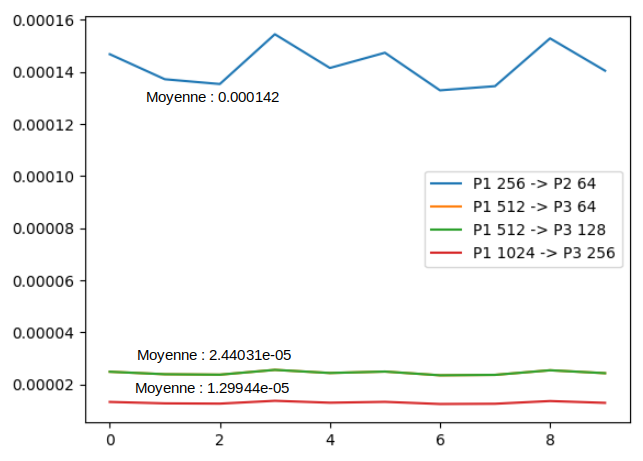
\includegraphics[width=0.7\linewidth]{test3_poly_3.png} 
\end{minipage}